% !TeX spellcheck = en_US
\chapter{Introduction}

\section{Units and Notation}
Throughout this work, a subset of the natural unit system will be used, as it is convention in high energy particle physics. The speed of light and the reduced Planck constant are fixed to $c = 1$ and $\hbar = 1$, and as such they are omitted in equations. Additionally, energy is expressed in \eV, where \unit{1}{\eV} is the energy gain of an electron which is accelerated across a \unit{1}{\volt} potential ($\unit{1}{\eV} \approx \unit{1.602 \e{-19}}{\joule}$). These conventions induce a change in units for the other dimensions, most importantly mass and momentum, both of which are notated in \GeV.

\section{The Standard Model}
The \emph{standard model} (SM) is a theory that represents our current knowledge of elementary particles, their forces and interactions, excluding gravity. 

Particles in the standard model can be classified into two separate classes: \emph{Fermions}, which make up matter and possess a spin of \nicefrac{1}{2}, and \emph{bosons}, which are mediators of forces and possess an integer spin.
Three elementary forces are predicted: \emph{electrodynamic} (Quantum Electrodynamics, QED), \emph{strong} (Quantum Chromo Dynamics, QCD) and \emph{weak} (Quantum Flavor Dynamics). The forces are induced by corresponding charge-like properties: electrodynamic charge, color charge and weak isospin. These charges can then be used to further subdivide fermions into \emph{quarks} and \emph{leptons} which will be described in the following sections. 

The standard model also provides theoretical predictions about the relations between particles, their masses and the probabilities of certain processes to happen. Because the probability is proportional to the number of times that a process occurs, experimentalists can validate the standard model by counting events with certain outcomes.

\subsection{Leptons}
There are three charged leptons: the \emph{electron} (\Pe), the \emph{muon} (\Pmu) and the \emph{tau} (\Ptau). They carry the electric charge of \unit{-1}{e} and participate in electrodynamic and weak interactions. For each charged lepton, there is one \emph{neutrino} counterpart (\Pnue, \Pnum, \Pnut). Neutrinos are electrically neutral, weakly interactive, light or massless particles. They remain undetected in current collider detectors.
The leptons do not carry color charge and are thus excluded from the strong interaction.
An overview about the leptons and their masses can be found in table~\ref{tbl:sm_leptons}.

\begin{table}[htbp]
	\center
	\begin{tabular}{ r | l | l | l | }
		\cline{2-4}
		& \multicolumn{3}{c|}{Leptons} \\ \cline{2-4}
		& electron (\Pe) & muon (\Pmu) & tau (\Ptau) \\ \cline{2-4}
		mass & \unit{511.0}{\keV} & \unit{105.7}{\MeV} & \unit{1.777}{\GeV} \\ \cline{2-4}
		charge & $-1$ & $-1$ & $-1$ \\ \cline{2-4}
		& \Pe neutrino (\Pnue) & \Pmu neutrino (\Pnum) & \Ptau neutrino (\Pnut) \\ \cline{2-4}
		mass & $< \unit{2}{\eV}$ & $< \unit{0.19}{\MeV}$ & $< \unit{18.2}{\MeV}$ \\ \cline{2-4}
		charge & 0 & 0 & 0 \\ \cline{2-4}
	\end{tabular}
	\caption{Leptons in the standard model\cite[p.~30, p.~690f.]{Oo2014Review}.}
	\label{tbl:sm_leptons}
\end{table}

\subsection{Quarks}
Similarly to the leptons, quarks can be divided into three generations. The first generation contains the stable \emph{up} and \emph{down} quarks, the second generation the \emph{charm} and \emph{strange} quarks and the third generation contains the heavy \emph{top} and \emph{bottom} quarks. Quarks carry a fractional electric charge of either \unit{\nicefrac{2}{3}}{e} or \unit{\nicefrac{-1}{3}}{e}.
They also carry color charges and take part in the strong interaction as well as in the weak interaction.
The three quark generations and their properties are shown in table~\ref{tbl:sm_quarks}.

\begin{table}[htbp]
	\center
	\begin{tabular}{ r | l | l | l | }
		\cline{2-4}
		& \multicolumn{3}{c|}{Quarks} \\ \cline{2-4} 
		& up (\Pup) & charm (\Pcharm) & top (\Ptop) \\ \cline{2-4}
		mass & \unit{2.3}{\MeV} & \unit{1.28}{\GeV} & \unit{173.2}{\GeV} \\ \cline{2-4}
		charge & \nicefrac{2}{3} & \nicefrac{2}{3} & \nicefrac{2}{3} \\ \cline{2-4}
		& down (\Pdown) & strange (\Pstrange) & bottom (\Pbottom) \\ \cline{2-4}
		mass & \unit{4.8}{\MeV} & \unit{95}{\MeV} & \unit{4}{\GeV} \\ \cline{2-4}
		charge & \nicefrac{-1}{3} & \nicefrac{-1}{3} & \nicefrac{-1}{3} \\ \cline{2-4}
	\end{tabular}
	\caption{Quarks in the standard model\cite[p.~33]{Oo2014Review}.}
	\label{tbl:sm_quarks}
\end{table}

\subsection{Bosons}
Gauge bosons are mediators of the elementary forces. QED is mediated by the massless \emph{photon} (\Pphoton), QCD by the massless \emph{gluon} (\Pgluon) and the weak interaction by the massive \PZ and \PWpm bosons. They couple to the corresponding charges. To account for the massive boson masses, the Higgs mechanism is introduced. The Higgs field gives rise to the Higgs boson (\PHiggs), a candidate of which has been found in 2012\cite{Ao2015Combined}.
All bosons and their properties are listed in table \ref{tbl:sm_bosons}.

\begin{table}[htbp]
	\center
	\begin{tabular}{ r | l | l | l | l | l |}
		\cline{2-6}
		& \multicolumn{5}{c|}{Bosons} \\ \cline{2-6} 
		& Photon (\Pgamma) & Gluon (\Pgluon) & Z-Boson (\PZ) & W-Bosons (\PWpm) & Higgs (\PHiggs) \\ \cline{2-6}
		mass & 0 & 0 & \unit{91.2}{\GeV} & \unit{80.4}{\GeV} & \unit{126}{\GeV} \\ \cline{2-6}
		charge & 0 & 0 & 0 & $\pm 1$ & 0 \\ \cline{2-6}
		interaction & QED & QCD & weak & weak & Higgs \\ \cline{2-6}
	\end{tabular}
	\caption{Bosons in the standard model\cite[p.~27]{Oo2014Review}.}
	\label{tbl:sm_bosons}
\end{table}

\subsection{Antiparticles}
For each SM particle, there exists one counterpart with the same mass but an opposite sign for all charge-like properties, called \emph{antiparticle}. Unlike fermions, bosons are their own antiparticles, called Majorana particles.

\section{The Large Hadron Collider}
Elementary particles and the standard model are commonly studied using scattering experiments. Two options arise: \emph{fixed target} and \emph{collider} experiments. Latter ones are preferred for high energies due to kinematic reasons.
A collider can be separated into two basic parts: an \emph{accelerator} and a \emph{detector}.
Inside the accelerator, the particles are accelerated to high energies using an electric field on a circular trajectory which is enforced by dipole magnets. Two beams are maintained, circulating in opposite directions, which are deflected inside the detectors positioned along the ring to produce collisions.

\begin{figure}[htbp]
	\center
	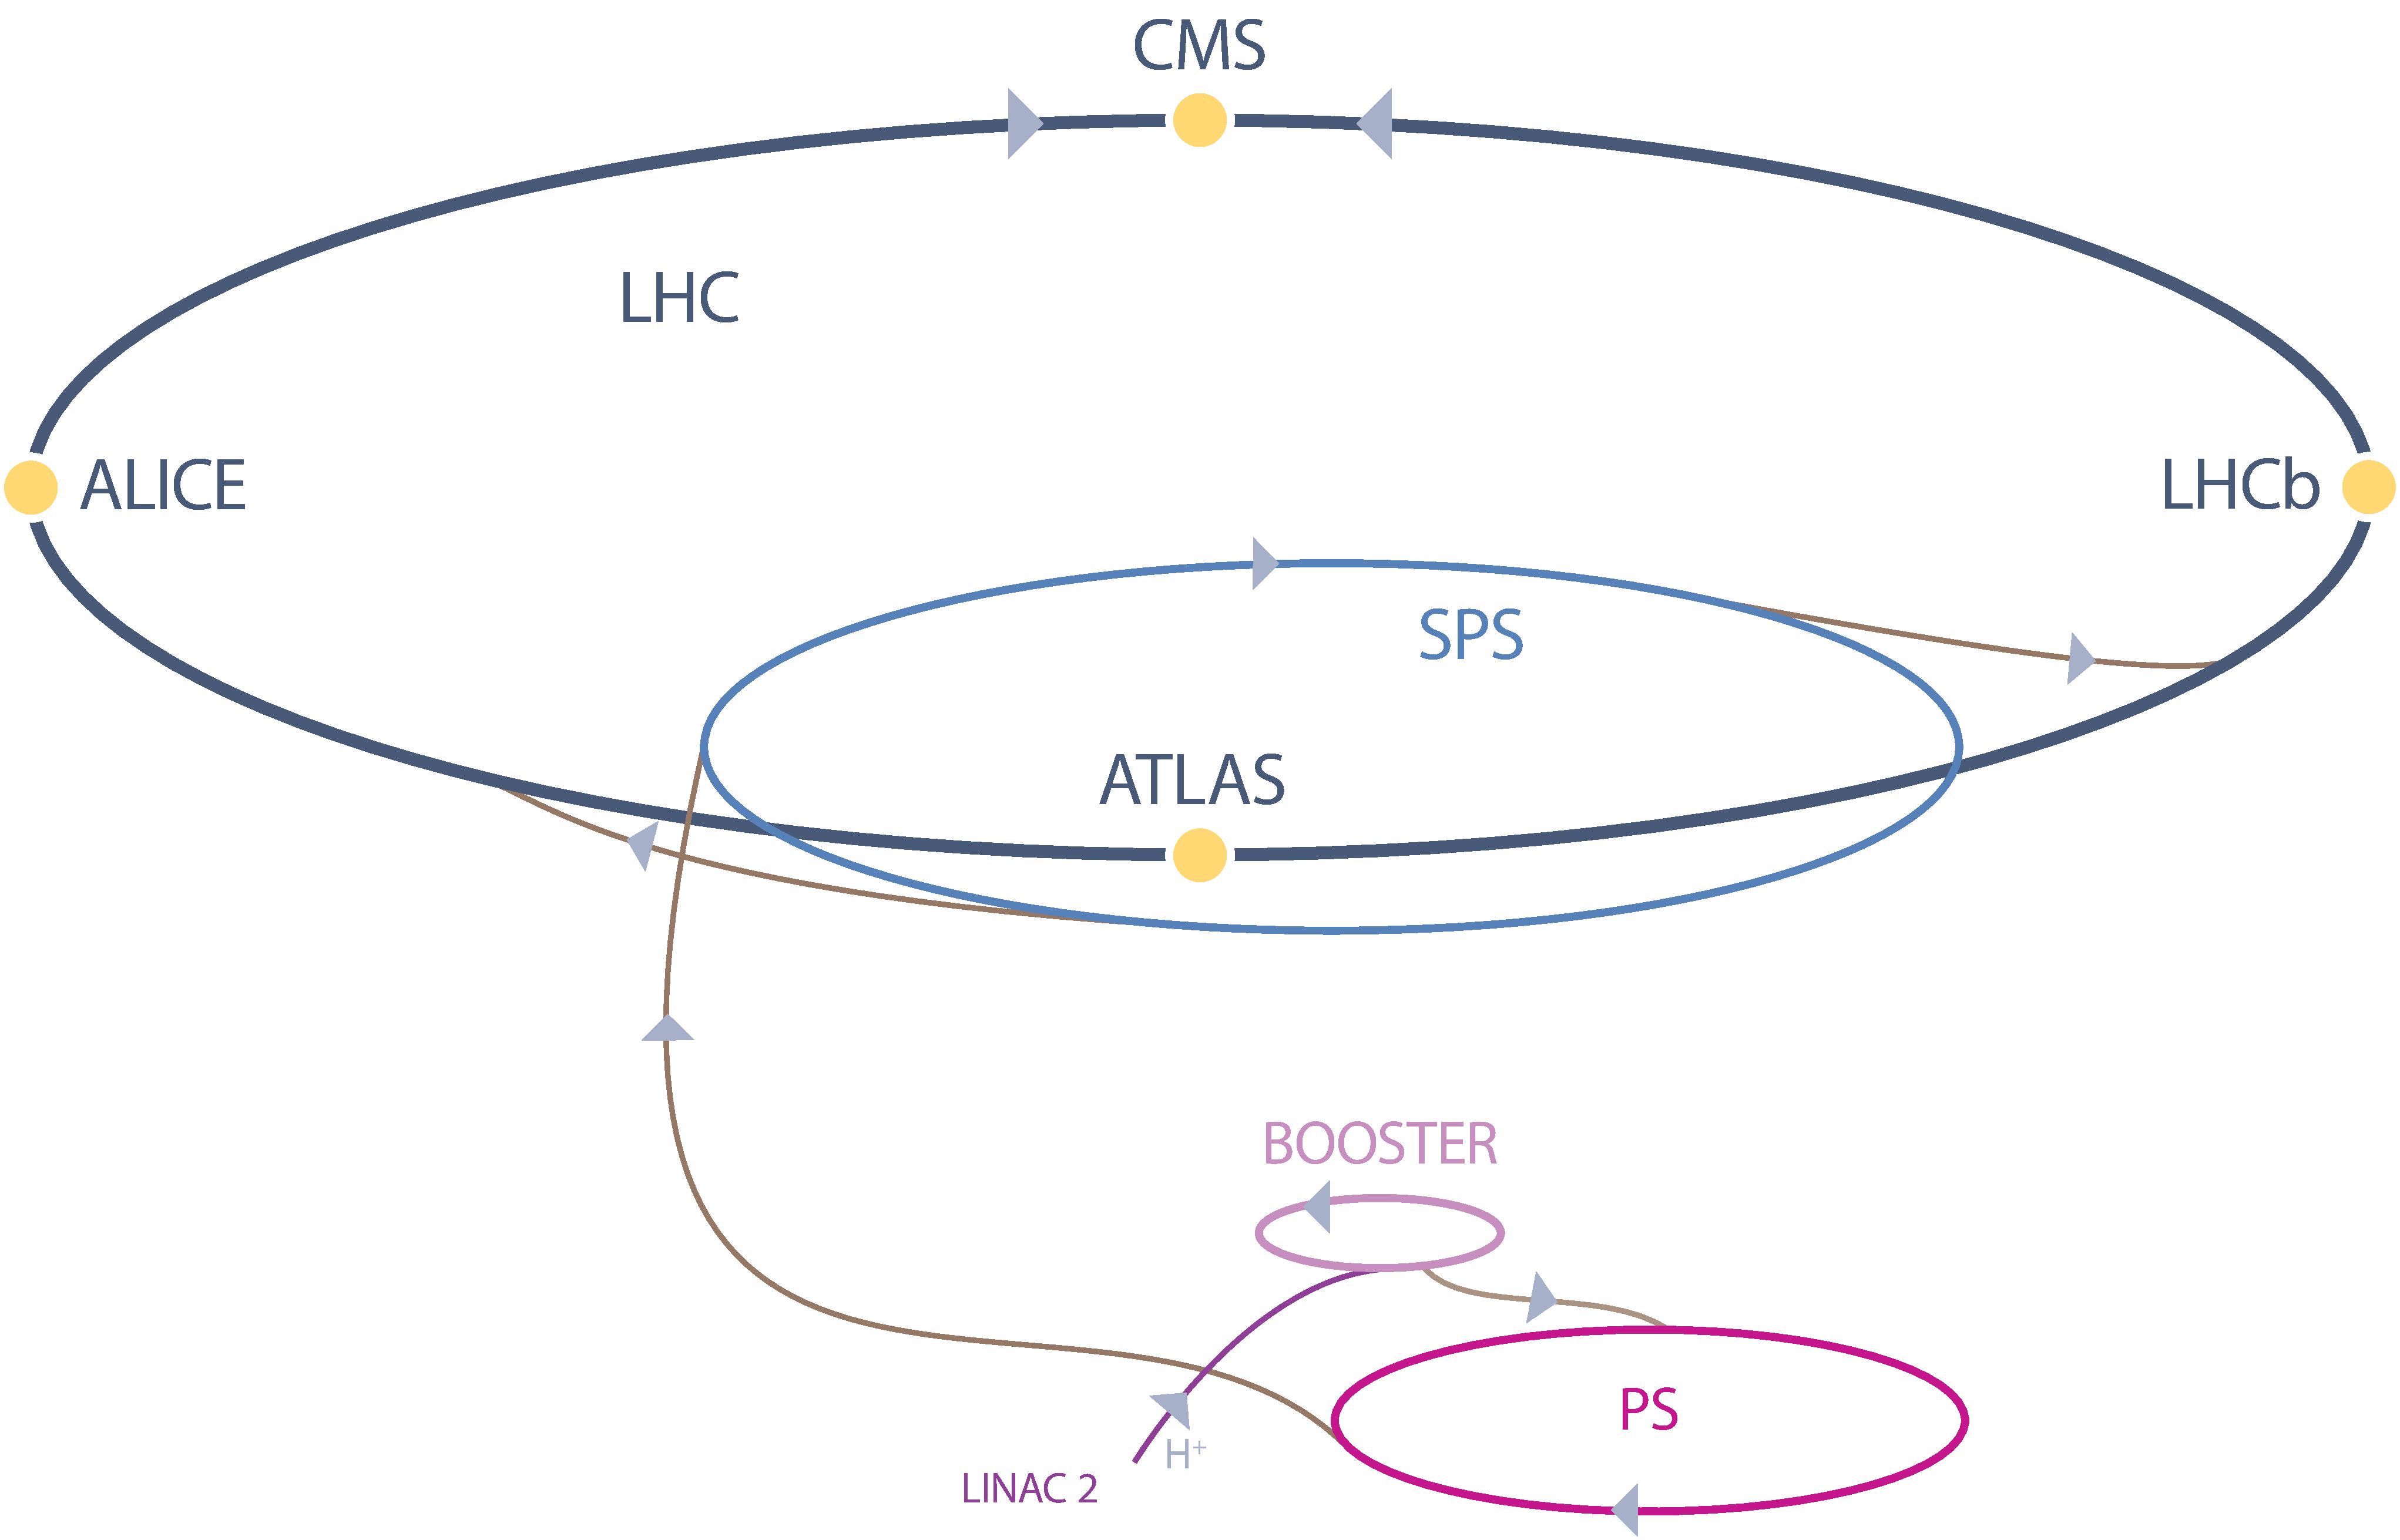
\includegraphics[width=0.5\textwidth]{CERN_accelerator_complex.pdf}
	\caption{The CERN accelerator complex\cite[modified]{Marcastel2013CERNs}. Shown are the LHC ring, the preaccelerators (Linear Accelerator 2, BOOSTER, Proton Synchrotron, Super Proton Synchrotron) and the four LHC experiments: CMS, ATLAS, ALICE and LHCb.}
	\label{fig:cern_accelerator_complex}
\end{figure}

The \emph{Large Hadron Collider} (LHC) is a proton-proton collider experiment of the European Organization for Nuclear Research (\emph{Conseil Européen pour la Recherche Nucléaire}, CERN), situated between \unit{45}{\meter} and \unit{170}{\meter} underground near Geneva, Switzerland. The LHC has been installed in the tunnel of the former LEP collider, having a circumference of \unit{26.7}{\kilo\meter}\cite{BV2009CERN,EB2008LHC}. The proton beams are injected after passing a series of preaccelerators, as shown in figure \ref{fig:cern_accelerator_complex}. It has been designed to provide an energy of \unit{7}{\TeV} per beam, resulting in a center-of-mass energy $\sqrt{s} = \unit{14}{\TeV}$. It is currently (2015) running at $\sqrt{s} = \unit{13}{\TeV}$, the data analyzed in this work was taken in 2012 with $\sqrt{s} = \unit{8}{\TeV}$.

\section{The Compact Muon Solenoid detector}
CMS is an experiment at the LHC. The CMS detector consist of a barrel section along the beam pipe, which is closed off by two end caps. Collisions happen in the center of the barrel at the interaction point. 
The detector parts and particle footprints can be found in figure \ref{fig:cms_slice}.
Close to the \emph{interaction point}, the inner part of the barrel contains a \emph{silicon tracker} used to record trajectories of charged particles. 
The inner tracker is surrounded by an \emph{electromagnetic calorimeter} (ECAL) made of lead tungstate crystals. The ECAL measures energy deposited by electrons and photons, combined with the tracker it can distinguish between the two particle types. 
After the electromagnetic calorimeter follows the \emph{hadron calorimeter} (HCAL). It is a sampling calorimeter composed of layers of brass absorber plates and plastic scintillator fibers. Due to the high density of the brass absorbers, hadronic showers deposit most of their energy inside the HCAL.
The HCAL is surrounded by the most important feature of the CMS detector, the \emph{solenoid magnet}. The solenoid coil is cooled down below \unit{10}{\kelvin}, where the NbTi (Niobium-titanium) conductor becomes superconducting, allowing for currents up to \unit{19}{\kilo\ampere}. The resulting field strength in the center of the coil is \unit{4}{\tesla}. The strong magnetic field causes the particle tracks to bend, this effect is used to measure the momentum of particles.
In the outer part one finds the iron return yoke interspersed with \emph{muon drift chambers}. Since only muons and neutrinos pass through the solenoid and iron yoke and neutrinos remain undetected, the drift chambers can precisely assess the muon momentum.\cite{Co2008CMS}

\begin{figure}[htbp]
	\center
	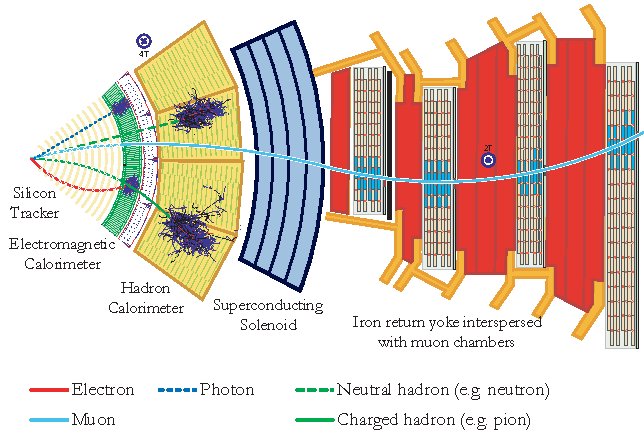
\includegraphics[width=\textwidth]{CMS_Slice.pdf}
	\caption{Slice through the CMS detector. The different detector layers (tracker, ECAL, HCAL, magnet, muon chambers) are shown, alongside schematic tracks of an electron, a photon, a charged and neutral hadron and a muon.\cite[modified]{Barney2011CMS}}
	\label{fig:cms_slice}
\end{figure}

\subsection{Coordinate System}
The CMS collaboration has defined a spherical coordinate system inside the detector, as illustrated in figure \ref{fig:cms_coordinate_system}. The origin is located in the interaction point, the z-axis points along the beam pipe towards the Jura mountains. The x-axis is defined towards the center of the LHC ring. An azimuthal angle $\phi$ is defined from the x-axis in the x-y plane. The polar angle $\theta$ is measured from the z-axis. One can also define a radial coordinate $r$ in the x-y plane, as distance from the z-axis.\cite[p. 2]{Co2008CMS} 

\begin{figure}[htbp]
	\center
	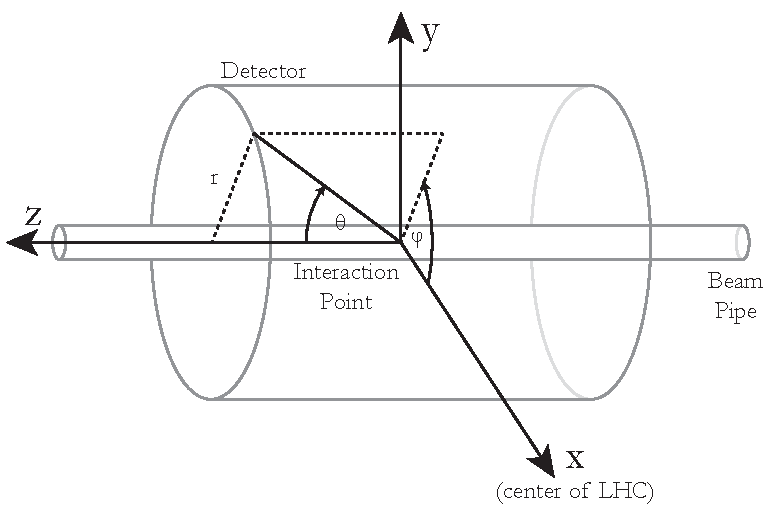
\includegraphics[width=0.6\textwidth]{CMS_coordinate_system.pdf}
	\caption{The CMS coordinate system.}
	\label{fig:cms_coordinate_system}
\end{figure}

\section{Commonly used quantities}
Since the particles initially move along the z-axis and only scatter partially, the exact longitudinal velocity of the center-of-momentum frame is unknown. 
Thus, most of the kinetic variables are defined in the transverse (x-y) plane. A particle is assigned a \emph{transverse momentum} \pT, which only contains the transverse component of its momentum vector. Analogous, only a fraction of the energy is regarded, the \emph{transverse energy} \ET. 
The sum of all transverse momenta in a final state is usually not equals to zero, since invisible neutrinos carry away some of the momentum. This is accounted for by the negative sum of the transverse energy, which is called \emph{missing transverse energy} \MET.
Another commonly used quantity is the pseudo-rapidity $\eta = -\ln \tan(\theta/2)$, which has the property that its distances are Lorentz invariant.

\section{Bunch crossings, events, collisions and pileup}
For practical acceleration purposes, the protons circulating in the LHC beam pipe are grouped into 2808 \emph{bunches}\cite[p.4]{EB2008LHC}. A \emph{bunch crossing} happens every \unit{50}{\nano\second} (2012), defining an \emph{event}. During an event, any number of hard collisions can occur. Events with multiple pp-collisions are called \emph{pileup} events.

\section{Trigger}
Since the raw data for each event is about $\order{\unit{1}{\mega\byte}}$, the throughput required to transfer all data would be $\order{\unit{20}{\tera\byte}}$ per second. This amount of data is too much for current hard- and software, thus a selection mechanism is introduced to match the amount of recorded data to the networking, processing and storage capabilities. This system is called \emph{trigger}. The CMS trigger system consists of two layers, the "Level-1 Trigger" (L1), implemented in hardware on site, and the software "High-Level-Trigger" (HLT), located at a computing farm close to the detector. For each run, the operator defines a set of selection requirements, called \emph{trigger menu}. These requirements reduce the data amount by $\order{10^{-6}}$.

\section{Event reconstruction}
In the \emph{reconstruction} (RECO) step, various algorithms are executed offline to reconstruct physics objects from the recorded data. The most important inputs are the bending radius of the particle tracks, energy deposits in the calorimeters and hits in the muon chambers. 
A notable algorithm that ensures that each input is linked to exactly one physics object has been developed by CMS and is called \emph{Particle-Flow}\cite{2009Particle}. 